\section{Introduksjon, begreper og IEC 61508}
\label{sec:intro}

\subsection{Funksjonell sikkerhet}

\textbf{Funksjonell sikkerhet dreier seg om sikkerhet som ivaretas av elektriske, elektroniske og programmerbare (E/E/EP) systemer slik at vi kan beskytte mennesker, miljø og infrastruktur fra skade}. Det er et system som utfører en aktiv sikkerhetsfunksjon ved \textbf{behov}, for eksempel et system som henter en båt inn igjen dersom avviket rapportert fra DP-systemet blir for stort. Sikkerhet definerer vi som fravær av uakseptabel risiko.


\subsection{Akronymer og begreper}

\begin{itemize}
    \item \textbf{SCS}: Safety Critical System
    \item \textbf{SIS}: Safety Instrumented System. System med flere SIF-er
    \item \textbf{SIF}: Safety Instrumented Function. The Safety Instrumented Function is a protection layer whose objective is to achieve or maintain a safe state of the process when a specific dangerous event occurs. The SIF is implemented in the SIS (Safety Instrumented System) which is normally composed of several Safety Functions.
    \item \textbf{SIL}: Safety Integrity Level
    \item \textbf{EUC}: Equipment Under Control
    \item \textbf{PFD}: Probability of Failure on Demand
    \item \textbf{PFH}: Probability of Failure per Hour
    \item \textbf{ALARP}: As low as reasonably possible. Et prinsipp som betyr at risiko alltid må reduseres så mye som praktisk mulig. I en risikovurdering kan det være ett tiltak som er teoretisk mulig for å redusere risiko, men som dessverre vil medføre for store kostnader i forhold til hvor mye risikoen reduseres. Og det kan da være helt greit i følge ALARP-prinsippet å ikke utføre tiltaket. Samtidig er man forpliktet til å utføre tiltak som reduserer risiko også selv om risikoen i utgangspunktet ikke framstår som spesielt alarmerende. Man er forpliktet så lenge kostnadene forbundet med tiltakene er akseptable i forhold til vinningen.
    \item \textbf{Hazard}: Potensiell farekilde forårsaket av at komponenten ikke utfører sin funksjon på en tilfredsstillende måte.
\end{itemize}


\subsection{Systemmodeller og metoder}

Vi sier at et system kan beskrives av fire aspekter. Vi bruker et enkelt gressklippe-eksempel for å illustrere.

\begin{itemize}
    \item \textbf{Systemets komposisjon}: Samlingen av delene og objektene i systemet. F. eks. personen og gressklipperen.
    \item \textbf{Miljøet}: Miljøet som systemet operer i. Det som er definert på utsiden av systemet men som både kan påvirke og bli påvirket av systemet. F. eks. plenen.
    \item \textbf{Systemets struktur}: Relasjonene mellom systementiteter som innehar en rolle i systemet, dvs aktører som har en aktiv rolle og kan ta avgjørelser, ha ansvar for måloppnåelse osv. F. eks. kontrollere, aktuatorer, sensorsystemer. F. eks. Personen som klipper plenen. OBS: En aktør kan være både del av komposisjonen og strukturen.
    \item \textbf{Systemets mekanismer}: Prosessene og funksjonene som gjør at systemet oppfører seg som det gjør. 
\end{itemize}

Disse kan illustreres i et \textit{systemtriangel}, hvor emergent oppførsel $\mu(s)$ oppstår i midten som resultat av samhandling mellom de tre hjørnene, og miljøet på utsiden.

\begin{figure}[H]
    \centering
        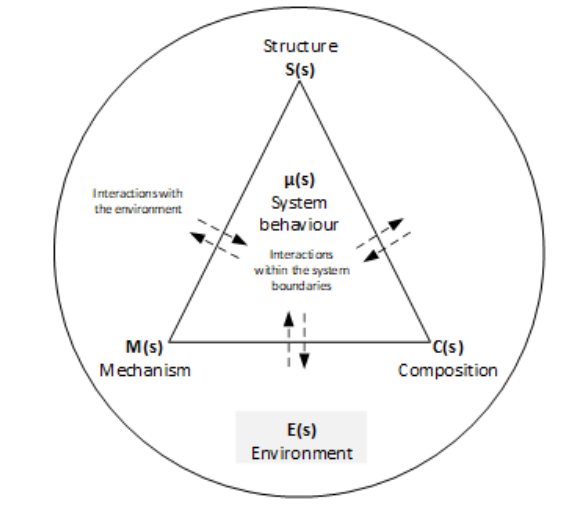
\includegraphics[width=0.7\textwidth]{figures/IEC/cesm.PNG}\\
        \caption{Illustrasjon av de ulike aspektene av CESM-modellen.}
\end{figure}

Aspektene i CESM er både nødvendig og tilstrekkelig for å forstå egenskapene og oppførselen til ethvert system.
For å finne en fullstendig modell av systemet, trenger vi systemmodeller som til sammen adresserer hele CESM metamodellen. Dette kan være vanskelig å få til.  Husk, George Box: Alle modeller er feil;
noen er nyttige, som også betyr at \textbf{ikke alle er nyttige}.

Flere systemmodeller kan representere hver av elementene i CESM. Dette står man fritt til å velge i forhold til
målsetting og situasjon. En "komplett" systemmodell kan dannes med basis i følgende modelltyper som hver for
seg adresserer forskjellige elementer i CESM:


\begin{itemize}
    \item Funksjonsmodell
    \item Aktørmodell
    \item Objektmodell
    \item Målmodell
    \item Modell(er) av oppførsel (emergens $\mu(s)$)
\end{itemize}

\begin{figure}[H]
    \centering
        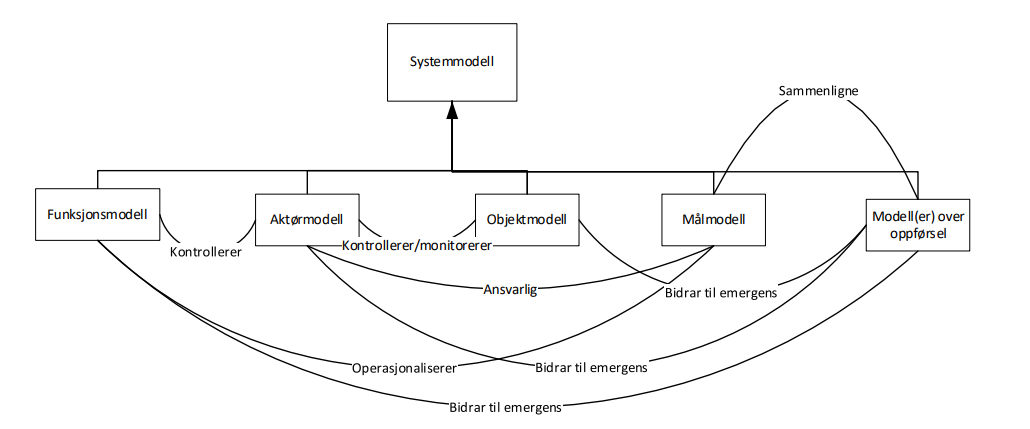
\includegraphics[width=\textwidth]{figures/IEC/systemmodell.PNG}\\
        \caption{Illustrasjon av hvordan de ulike modellene henger sammen, for å beskrive alle elementene i CESM.}
\end{figure}

\subsection{IEC61508}

\textbf{IEC61508} er en internasjonal standard som inneholder krav og analyser for funksjonell sikkerhet.



\subsection{Sikkerhets Livssykel (Safety Lifecycle)}

IEC 61508 definerer livssykelen til et sikkerhetssystem i 16 faser.

\begin{itemize}
    \item[\textbf{1:}] Konsept:  Her defineres EUC og EUC Control System
    \item[\textbf{2:}] Scope definisjon: Avgrensning. Avdekke sentrale krav, operasjonelle antakelser, erfaringer fra tidligere som er nyttig for neste fase.
    \item[\textbf{3:}] Hazard og risiko analyse for EUC og EUC control system. Hazard vil si en farekilde som er en egenskap ved systemet, for eksempel høyt trykk. Først identifiserer man potensielle hazardous events (ofte i en workshop ved hjelp av sjekklister og/eller en strukturert analyse), før man analyserer disse tilfellene i en risikotabell, se tabell under.
    \item[\textbf{4:}] Generelle sikkerhetskrav: Liste sikkerhetskrav av overordnede funksjoner og tiltak som risikoanalysen har avdekket.
    \item[\textbf{5:}] Allokere sikkerhetskrav. Fra risikoanalysen og de risikoreduserende tiltakene får vi formelle krav til sikkerhetssystemet, i tillegg til prioritering og pålitelighetsbehov. 
    
    \textbf{1} - Bestemme hvilke systemer som skal utføre hvilke funksjoner. Skal det være organisatoriske tiltak, menneskelige aksjoner eller aksjoner utført av tekniske systemer som SIS? Og for SIS: Skal funksjonene plasseres i samme SIS, eller i flere SIS?
    
    \textbf{2} - Bestemme pålitelighetskrav til funksjoner som skal utføres av SIS(er) og tilhørende SIL-krav. Pålitelighetskrav kan for eksempel være en gitt PFD og/eller PFH, altså en gitt sannsynlighet for feil og/eller forventet hyppighet av feilen. Merk: Pålitelighetsmålet PFD brukes for SIFer som er low-demand (behov for disse sjeldnere enn en gang i året), mens PFH (frekvens av farlige feil per time) benyttes som pålitelighetsmål for SIFer som er «high-demand/ «continous demand», det vl si hhv behov for oftere enn en gang i året eller kontinuerlig. Vi spør oss altså: Hvor sannsynlig er feilen, eller hvor ofte kan den oppstå?
    
    \item[\textbf{6-8:}] ...
    \item[\textbf{9-10:}] Designe SIS og SIF-er i henhold til SIL krav. Hvor pålitelige skal de være? Hvor skal sikkerhetsfunksjonen plasseres?
    \item[\textbf{11-16:}] ...

\end{itemize}

\begin{table}[]
\begin{tabular}{|l|l|l|l|l|l|l|}
\hline
\begin{tabular}[c]{@{}l@{}}Farlig\\ hendelse\end{tabular}                                                                        & Årsak(er)                                                                                  & \begin{tabular}[c]{@{}l@{}}Worst\\ case\\ konsekvens\end{tabular}                                  & \begin{tabular}[c]{@{}l@{}}Alvorlighet\\ Farlig\\ Hendelse\end{tabular}          & \begin{tabular}[c]{@{}l@{}}Alvorlighet\\ Konsekvens\end{tabular}                 & Risiko                                                                                                                                   & \begin{tabular}[c]{@{}l@{}}Risiko-\\ reduserende\\ tiltak\end{tabular}                                  \\ \hline
\begin{tabular}[c]{@{}l@{}}En hendelse\\ som kan\\ lede til\\ ulykke om\\ den ikke\\ forhindres\\ eller\\ begrenses\end{tabular} & \begin{tabular}[c]{@{}l@{}}Farekilder\\ og\\ triggere\\ (initiating\\ events)\end{tabular} & \begin{tabular}[c]{@{}l@{}}Mhp.\\ personskade,\\ miljø\\ eller\\ materielle\\ verdier\end{tabular} & \begin{tabular}[c]{@{}l@{}}Kategori\\ valgt\\ fra risiko-\\ matrise\end{tabular} & \begin{tabular}[c]{@{}l@{}}Kategori\\ valgt\\ fra risiko-\\ matrise\end{tabular} & \begin{tabular}[c]{@{}l@{}}Enten en\\ score, eller\\ eksempelvis\\ høy (uakseptabel)\\ middels (ALARP)\\ lav (neglisjerbar)\end{tabular} & \begin{tabular}[c]{@{}l@{}}Tekniske,\\ organisatoriske,\\ og/eller\\ menneskelige\\ tiltak\end{tabular} \\ \hline
\end{tabular}
\end{table}

Safety lifecycle utviklingsmetoden skiller seg fra andre metoder ved at det er en risikobasert tilnærming for å sille krav. Man får krav til risikoreduserende tiltak og pålitelighetskrav for SIF-er og SIL-krav. Designprosessen og detaljkravene for realisering blir så styrt av SIL-kravet. SIL-kravet må også følges opp i driftsfasen.

Et eksempel på et risikoreduserende tiltak er å introdusere redundans i systemet, med flere av samme komponent og votering.

\subsection{Bowtie-modellen}

Bowtie-modellen kan brukes for å analysere farlige hendelser og for å plassere sikkerhetstiltak. Den kan også brukes for å identifisere hvor det er behov for SIS og SIFer.

\begin{figure}[H]
    \centering
        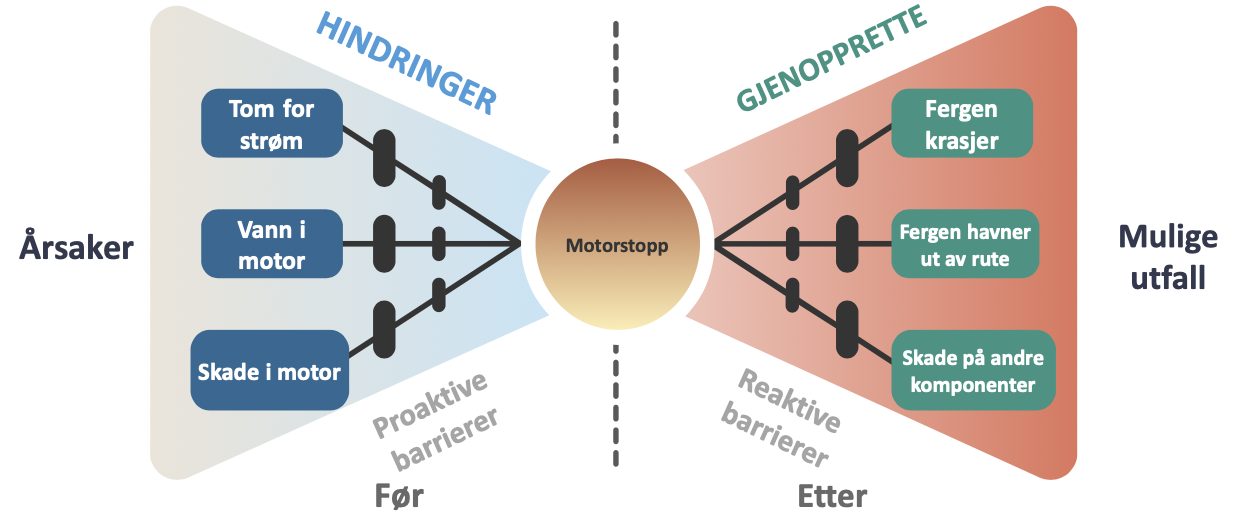
\includegraphics[width=\textwidth]{figures/IEC/bowtie.png}\\
        \caption{Bowtie-analyse for den farlige hendelsen motorstopp.}
\end{figure}

\subsection{SIL-krav}

Et SIL-krav er et krav om at SIF-en vi designer \textit{må} ha PFD og PFH tilsvarende et bestemt SIL-nivå. Høyt SIL-nivå tilsvarer lav sannsynlighet og hyppighet for feil, og vil da indikere en relativt sikker SIF. Lavt SIL-nivå indikerer en mindre sikker komponent og man vil da ofte implementere f. eks. redundans ved votering.
 
For å kunne oppfylle kravene må en ha gjennomført en analyse og klassifisering av de feilene som er registrert på tilsvarende komponenter. For nytt utstyr må en gjøre en analyse (FMEDA – Failure Mode and Diagnosis Analysis) av komponenten for å kunne kvantifisere de forskjellige feilmodiene. Spesielt er det viktig å finne de farlige udetekterte feilene (DU- Dangerous Undetected) som angis med $\lambda_{DU}$ [feil per time].

SIL-kravet får implikasjoner for designet av systemet. Det gir blant annet krav til 

\begin{itemize}
    \item Redundans/votering (per delsystem) ved å stille krav til minimum feiltoleranse.
    \item Krav til diagnostic coverage (evne til å avdekke farlige feil vha diagnostikk: hvor ofte forventer vi å klare å finne feil, og stille riktig diagnose?
    \item Restriksjoner for valg av programmeringsspråk og krav til funksjonalitet i programmeringsverktøy
    \item Krav til at beregnet PFD/PFH for hele SIFen er innenfor SIL-kravet. Dette vil implisitt gi øvre grenser for feilrater for farlige feil, både detekterte og udetekterte, hvor ofte funksjonen testes for å avdekke farlige udetekterte feil, og hvor lang reparasjonstid ifbm farlig detekterte feil.
\end{itemize}

Et eksempel på en SIF og tilhørende SIL-krav:
Fra risikoanalyse og allokering har vi funnet at vi trenger en SIF i form av en av/på-ventil som stenger dersom trykket i tanken blir for høyt. Da trenger vi følgende komponenter:

\begin{itemize}
    \item Sensor
    \item Logisk enhet
    \item Av/på-ventil
\end{itemize}

Fra risikoanalysen ble det funnet at hele SIFen må ha SIL-krav 2. OBS: PFD/PFH skal summeres for alle komponentene som inngår i SIF-en.

\begin{figure}[H]
    \centering
        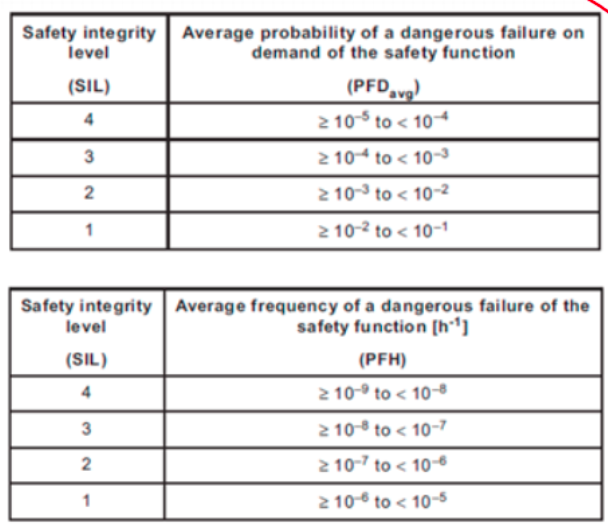
\includegraphics[width=\textwidth]{figures/IEC/sil.png}\\
        \caption{SIL-nivå}
\end{figure}

\subsection{Hvor mye risiko skal vi tillate?}

\begin{figure}[H]
    \centering
        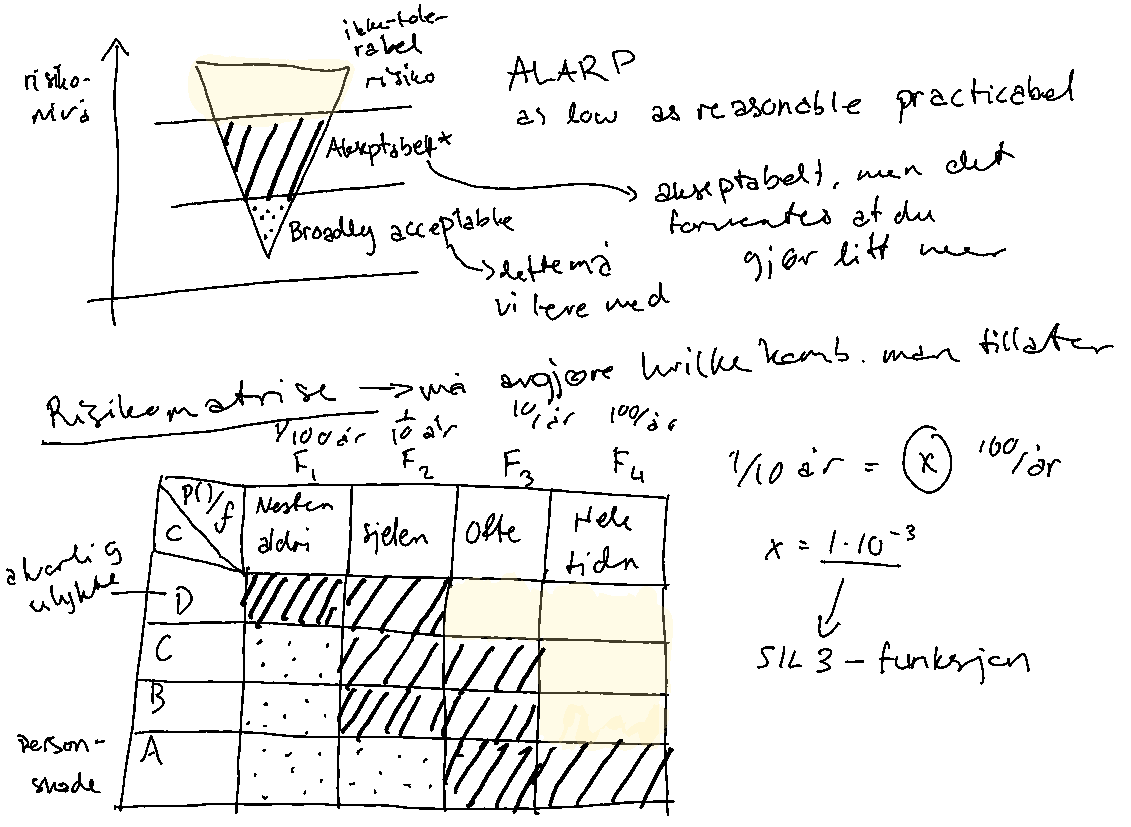
\includegraphics[width=\textwidth]{figures/IEC/risikomatrise.png}\\
        \caption{Risikonivå og risikomatrise. C er farekategori for konsekvens av den farlige hendelsen.}
\end{figure}
